\section{IP ADRESİ VE HESAPLAMALARI} %Notlarda 27.sayfa

32 bit uzunluğa sahip olan IP adresi 2 temel bileşene sahiptir. 

\begin{enumerate}
\item Ağ tanımlayıcı
\item Host tanımlayıcı
\end{enumerate}

\textbf{NOT : }Bir ağ içerisinde IP atanabilen ve kendisinin ağa bağlanma ihtiyacı olan bilgisayar, yönlendirici, güvenlik duvarı vb. cihazların tümüne host denir. 

IP adresinin bu iki bileşeni hesaplanırken alt ağ maskesine ihtiyaç duyulur. Temel olarak alt ağ maskesi IP adresinin sınıfına göre belirlenir. IP adresleri 32 bitin sekizerli olarak gruplandırılması ve decimal olarak gösterilmesi şeklinde olur. Bu 8 bitlik grupların her birine oktet denir. Her oktet birbirinden nokta ile ayrılır. 

\textbf{ÖRNEK : }
\begin{center}
\begin{tabular}{cccc}
00001010.&00000000.&00000001.&10000000 \\
10.       & 0.      & 1.      & 128      \\
Her sekizerli & & & \\
grup bir oktet & & &
\end{tabular}
\end{center}

Bir IP adresinin bağlı olduğu sınıf ilk oktetinden anlaşılır. 

\begin{center}
\begin{tabular}{cc}
00001010.00000000.00000001.&10000000 \\
ağ tanımlayıcısı           &  host tanımlayıcısı \\ 
24 bit ile $2^{24}$ tane ağ tanımlanabilir & 8 bit ile $2^8=256$ tane ağ tanımlanabilir\\
\end{tabular}
\end{center}

\textbf{ÖRNEK : } 16 tane IP adresini bölüyoruz. (${2^4}$ bit ) 

\begin{figure}[!ht] \centering 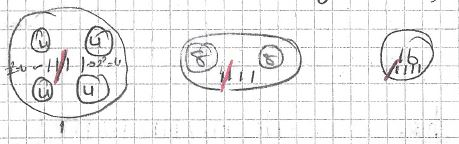
\includegraphics[width=10cm]{images/gorsel28sayfa} \label{fig:gorsel} \end{figure}

\textbf{NOT : }Ağlardaki bilgisayar sayıları(kullanılabilecek ip sayıları) belirlenirken maksimum kapasite 2'nin kuvveti ${2^n}$ %katı yazılmıştı, kuvveti olarak değiştirdim
alınarak belirlenir. 

\textbf{ÖRNEK : }Bir şirketin iki farklı şubesinde 120 ve 280 adet bilgisayar kullanılmaktadır. Bu şirketler için optimal ağ büyüklüklerini hesaplayınız. 

\begin{itemize}
\item[]$120 => 2^n = 2^7 => 128$
\item[]$280 => 2^n = 2^9 => 512$
\end{itemize}

\textbf{NOT : }Host tanımlayıcısı kısmında belirtilen bitlerde elde edilebilecek en büyük sayı o ağda kullanılabilecek IP adresi sayısıdır. Her ağın ilk IP adresi \underline{"ağ adresi"} ve son IP adresi \underline{"yayın adresi"} olarak kullanıldığından her ağda kullanılabilecek host sayısı IP sayısından 2 eksiktir.
\begin{itemize}
\item[] Host bitleri : n tane 
\item[] Ağdaki IP adresi : $2^n$ tane 
\item[] Ağda kullanılabilecek host sayısı $2^n-2$
\end{itemize}

\textbf{ÖRNEK : } 10.9.8.0 IP adresinin 30. bitten sonrasının bulunduğunu varsayalım. Alt ağ IP adresinin kullanım amacına göre yazalım. 

\begin{tabular}{ll}
..... & ..... \\
30 bit& 2bit\\
\end{tabular}

IP sayısı $2^2=4$ tane
Host sayısı $2^2-2=2$ tane


\begin{tabular}{lll}
1.IP adresi 10.9.8.0 & ->& Ağ adresi \\
2. ve 3. IP adresi 10.9.8.1 ve 10.9.8.2 & -> & Hostlar için kullanılabilir \\
4. IP adresi 10.9.8.3 & -> & Yayın adresi 
\end{tabular}

\textbf{NOT : }

\begin{tabular}{ll|l}
Ağ sayısı & Host sayısı &Toplam host sayısı\\
\hline 
1&16&14 \\
2 & 8 & $2(8-2) =12$ \\
4&4&$4(4-2) = 8$ \\
\end{tabular}


\subsection{IP Sınıfları}
IP'nin ilk tasarlandığı sıralarda ortaya çıkmış bir kavramdır. Kurumlarda IP adresleri tahsis edilirken ihtiyaca göre optimal sayıda verebilmek için tasarlanmıştır. En büyük IP sınıfı A sınıfı, en küçük IP sınıfı C sınıfıdır. 

\underline{A sınıfı :} İlk biti(MSB) 0 olan IP adresleridir. 

\begin{tabular}{l}
01111111.11111111.11111111.11111111 \\
  127  \hspace{1.1cm} 255\hspace{1.1cm}255\hspace{1.1cm} 255 \\
\end{tabular}

İlk oktet 0-127 arasında olur. Varsayılan ap maskesi 255.0.0.0'dır. A sınıfı bir IP adresinde $2^{24}$ tane IP oluşturulabilir.

\underline{B sınıfı} İlk iki biti 1.0 şeklindedir. Ondalık formda ilk  okteti 128 ve 191 arasındaki adreslerdir. Varsayılan alt ağ maskesi 255.255.0.0'dır. B sınıfı bir IP adresinde $2^{16}$ tane IP oluşturulabilir.


\underline{C sınıfı} İlk üç biti 1.1.0 şeklindedir. Ondalık formda ilk okteti 192 ve 223 arasındaki adreslerdir. Varsayılan alt ağ maskesi 255.255.255.0'dır. B sınıfı bir IP adresinde $2^{8}$ tane IP oluşturulabilir.

\underline{D sınıfı} İlk dört biti 1.1.1.0'dır. Ondalık formda ilk okteti 224-239 arasındadır. \underline{Multicast}(Çoklu yayın) olarak bilinir. Normalde hostlarda kullanılmaz. 

\underline{E sınıfı} 240-248 ile başlar. Deneysel amaçlar için rezerve edilmiştir. Normalde hostlarda ve ağlarda kullanılmaz.

\begin{tabular}{lll}
A sınıfı & 0-127 & \\
B sınıfı & 128-191 & \\
C sınıfı & 192-223 & \\
D sınıfı & 224.0.0.0 \vline & Kullanmıyoruz \\
E sınıfı & 255.0.0.0 \vline  &Kullanmıyoruz \\
\end{tabular} 

Peki neden böyle bir sınıflandırma yapıldı?

\begin{tabular}{l|l|l}
Ağ biti & Host bitleri & Her ağdaki IP sayısı \\
\hline
8& 24->A sınıfı &$2^{24}$ tane IP \\
16& 16->B sınıfı &$2^{16}$ tane IP \\
24&8->C sınıfı &$2^8$ tane IP \\

\end{tabular}

\textbf{ÖRNEK : } 132.x.x.x IP adresi B sınıfıdır.
132.45.x.x IP adresinin ilk iki okteti ağ tanımlayıcısı son iki oktet host tanımlayıcısıdır. $2^16$ tane IP alabilir. 

112.x.x.x IP adresi A sınıfıdır. $2^{24}$ tane IP alabilir.

193.140.253.x IP adresi C sınıfıdır. $2^8$ tane IP alabilir.


\subsection{Özel IP Adresleri(Private IP Blocks)}

İnternette kullanılmayan IP adresleridir. İnternet üzerinde hiçbir yönlendirici tarafından yönlendirilmeyen IP adresleridir. Bu adreslerin kullanım amacı test uygulamaları ve NAT uygulamaları gibi durumlardır. IP adresleri tükendiğinden kurumlarda kullanılan bilgisayarların tamamına yetmemektedir. Bu nedenle günümüzde kurumların iç ağlarında özel IP adresleri istenilen sayıda kullanılabilir. 

\begin{itemize}
\item 10.0.0.0/8 ->$2^{24}$ IP adresi
\item 172.16.0.0 ->$2^{20}$ IP adresi
\item 192.168.0.0 ->$2^{16}$ IP adresi
\end{itemize}

\textbf{NAT(Network Address Translation)}

\begin{figure}[!ht] \centering 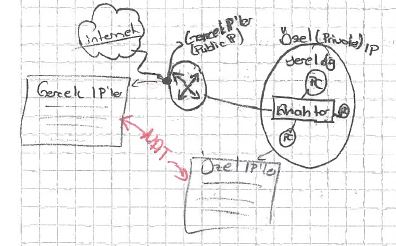
\includegraphics[width=10cm]{images/gorsel31sayfa} \label{fig:NAT} \end{figure}


\subsection{Ağ Maskesi(Netmask)}

IP adreslerinin bitlerden oluştuğunu ve iki bileşeni olduğunu biliyoruz. Bu iki bileşenin hangi bitten ayrılacağını bulmak için ağ maskesi kullanılır. Ağ maskesi herhangi bir IP adresi ile ikilik sistemde çarpılırsa(ve işlemi) çıkan sonuç ağın adresini verir. 


\textbf{ÖRNEK : }

\begin{itemize}
\item[] IP : 192.168.1.75
\item[] Ağ maskesi : 255.255.255.0
\item[] 11000000.10101000.00000001.01001011
\item[] 11111111.11111111.11111111.00000000
\item[] 11000000.10101000.00000001.00000000
\item[] Ağ adresi 192.168.1.0
\end{itemize} 

\subsection{CIDR Notasyonu}

Elimizde sadece IP adresleri olduğunda ağla ilgili yeterli bilgiye ulaşamadığımızı, ilave olarak IP adresinin hangi bitten bölündüğünü bilmemiz gerektiğini biliyoruz. Bunun için ağ maskesine alternatif olarak CIDR Notasyonu kullanılmaktadır. Bu gösterim şeklinde IP adresinin sağına "/" işareti konulup bölünen bit numarası yazılır. 

\textbf{ÖRNEK : } 

\begin{itemize}
\item[] 192.168.1.75 IP adresli ve 255.255.255.0 ağ maskesine sahip bir cihazın CIDR notasyonu 192.168.1.75/24 şeklindedir. 
\item[] 10.1.0.0 ve 255.0.0.0 ise 10.1.0.0/8 olarak gösterilir. 
\item[] 10.9.8.0 ve 255.255.255.128 ise 10.9.8.0/25 şeklinde gösterilir. (128 ikilik tabanda 10000000 şeklinde gösterildiğinden soldan 25 tane 0 vardır.) 
\end{itemize}

\subsection{Alt Ağa Bölme}
IP adresi ve ağı temsil eden bit sayısı belirli olan bir ağ birden fazla küçük ağlara bölünebilir. Alt ağa bölme işlemi alt ağ maskesinde bir bit kaydırılarak yapılır. Bu şekilde $2^n$ tane alt ağ bölme işlemi yapılabilir. 

\textbf{ÖRNEK : } 

\textbf{a)} 10.0.0.0/24 ağını iki ayrı ağa bölünüz.



\textbf{b)}Yeni oluşturulan ağlar için 10.0.0.100 ve 10.0.0.150 IP adreslerinin aynı ağda olup olmadıklarını hesaplayın. (İpucu : Ağ adresi = IP x Ağ maskesi)

\textbf{c)}128 IP'li ağların her birini ikiye bölünüz. 


\underline{Çözüm :}

\textbf{a)}
\begin{itemize}
\item[] Ağ : 10.0.0.0/24
\item[] Ağ maskesi : 255.255.255.0 (24 tane 1, 8 tane 0 var. $2^8$ tane IP var)
\item[] Ağ maskesi : 11111111.11111111.11111111.00000000 ağ maskesinde 1 bit sağa kaydırdığımızda 25 tane 1, 7 tane 0 olacaktır. $2^7=128$ tane IP elde edilir. 
\end{itemize} 

1 bit kayarsa $2^1=2$ alt ağ,
2 bit kayarsa $2^2=4$ alt ağ,
$\hdots$
,n bit kayarsa $2^n$ alt ağ elde edilebilir. 

10.0.0.0/25 notasyonuna sahip bir ağda 1.alt ağ 10.0.0.0 IP adresiyle başlar. 128 adet IP tanımlanır. Son IP 10.0.0.127 olur. 2. alt ağ ise 10.0.0.128 IP adresinden 10.0.0.255 IP adresine kadar 128 adet IP alabilir. 


\begin{tabular}{l|l|l|l|l|l}
&Ağ adresi & Yayın adresi & Ağ maskesi & IP sayısı & Host sayısı\\
\hline
1.ağ & 10.0.0.0/25 & 10.0.0.127 & 255.255.255.128 & 128 &126 \\
\hline
2.ağ & 10.0.0.128/25 & 10.0.0.255 &255.255.255.128 & 128 & 126 \\

\end{tabular}


\textbf{b)}

\begin{tabular}{llll}
& 00001001.00000000.00000000.01100100 &=& 10.0.0.100\\
ağ maskesi:& 11111111.11111111.11111111.00000000 &=&10.0.0.128\\
\hline
&00001001.00000000.00000000.10010110 &=&10.0.0.150 \\

\end{tabular}

Son oktetleri farklı olacağından aynı ağda değillerdir. 

\textbf{c)} 

\begin{tabular}{cc}
1.ağ & 2.ağ \\
\hline
10.0.0.0/25 & 10.0.0.128/25 \\
\end{tabular}

Ağ maskesi 255.255.255.128 

1111111.11111111.11111111.10000000

Yeni oluşan ağ maskesi 255.255.255.192

\begin{tabular}{ll}
1.ağ & \begin{tabular}{l}
10.0.0.0 ->ağ \\
\hline
10.0.0.63 ->yayın \\
\end{tabular}  \\   
\end{tabular}

\begin{tabular}{ll}
2.ağ & \begin{tabular}{l}
10.0.0.64 ->ağ \\
\hline
10.0.0.127 ->yayın \\
\end{tabular}  \\   
\end{tabular}



\begin{tabular}{ll}
3.ağ & \begin{tabular}{l}
10.0.0.128 ->ağ \\
\hline
10.0.0.191 ->yayın \\
\end{tabular}  \\   
\end{tabular}


\begin{tabular}{ll}
4.ağ & \begin{tabular}{l}
10.0.0.192 ->ağ \\
\hline
10.0.0.255 ->yayın \\
\end{tabular}  \\    
\end{tabular}

\textbf{SORU : } 10.9.6.0/25 ağını 4 ayrı ağa bölünüz.

Ağ maskesi 255.255.255.0
11111111.11111111.11111111.0

\begin{tabular}{lll}
Yeni ağ maskesi  & : &11111111.11111111.11111111.11100000 ($2^5=32$ IP var.) \\
                 & : & 255.255.255.224   \\
\end{tabular}

\begin{tabular}{cc}
\begin{tabular}{|cc|}
\hline 
10.0.0.0 & 10.0.0.64 \\
10.0.0.31 & 10.0.0.127\\
\hline 

\end{tabular}
&
\begin{tabular}{|cc|}
\hline 
10.0.0.32 & 10.0.0.128 \\
10.0.0.63 & 10.0.0.191 \\
\hline 
\end{tabular} \\
\end{tabular}

\textbf{ÖRNEK : } 10.0.0.0/22'yi 4 alt ağa bölünüz. 

11111111.11111111.11111100.00000000 $2^{10}=1024$ tane IP var. 

Ağ maskesi : 255.255.252.0

Yeni alt ağ maskesi : 255.255.255.0(2 bit kaydı.$2^{8}=256$ IP var.)

Yeni CIDR gösterimi -> 10.0.0.0/24 olmalıdır.

10.0.0.0 -> 10.0.0.255

10.0.1.0 -> 10.0.1.255

10.0.2.0 -> 10.0.2.255

10.0.3.0 -> 10.0.3.255

\textbf{ÖRNEK : } /17 şeklinde gösterilen ağın maskesi nedir?

11111111.11111111.10000000.00000000  = 255.255.128.0 şeklindedir. 

\textbf{ÖRNEK : } 10.10.0.0 ve 255.255.0.0 şeklindeki ağda kaç host olabilir?

$2^{16}-2$ adet host olabilir. 

\textbf{NOT : } Özel IP ile ??? 127 ile başlayan IP ler kullanılamazlar.  Localhost : 127.0.0.1 bilgisayarın kendisini temsil eder. 

169.254.0.0 Windows işletim sisteminin IP alınamadığında kendi IP bloğundan otomatik olarak verdiği IP adresidir. 


\textbf{ÖRNEK : } Bir şirkete 192.168.100.0/24 şeklinde IP aralığı tahsis edilmiştir. Şekilde sistem yöneticisi ağdaki aşırı yayın trafiğinin sorun çıkardığını düşünerek ağı alt ağlara bölmek istiyor. Birimlerin PC sayısı aşağıdaki gibidir. Teknik birim=70, Pazarlama=40, Muhasebe=20, İdari birim=25  

\begin{figure}[!ht] \centering 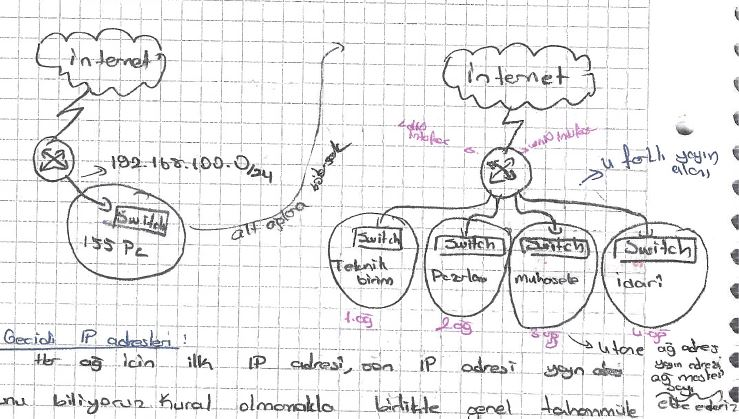
\includegraphics[width=10cm]{
images/sayfa36} \label{fig:Şirket örneği 1} \end{figure}

\subsection{Ağ Geçidi IP Adresleri }

Her ağ için ilk IP adresi ağ adresi, son IP adresi yayın adresi olduğunu biliyoruz. Kural olmamakla birlikte genel teamüllere göre ağ adresinden sonraki ilk IP adresi(kullanılabilecek ilk host adresi) ağ geçidi olarak belirlenir. Herhangi bir host adresi ağ geçidi olarak belirlensede hiçbir problem  olmaz. 

\textbf{NOT : } IP adresinin ve ağın son IP adresi değiştirilemez. 

\textbf{NOT : } Ağ geçidi IP adresi herbir ağın doğrudan bağlı olduğu yönlendirici arayüzünde(interface, ara birim, ethernet kartı, NIC(Network Interface Card)) tanımlı olan IP adresi olmak zorundadır. 

Günümüzde kullanılışı : 

\begin{figure}[!ht] \centering 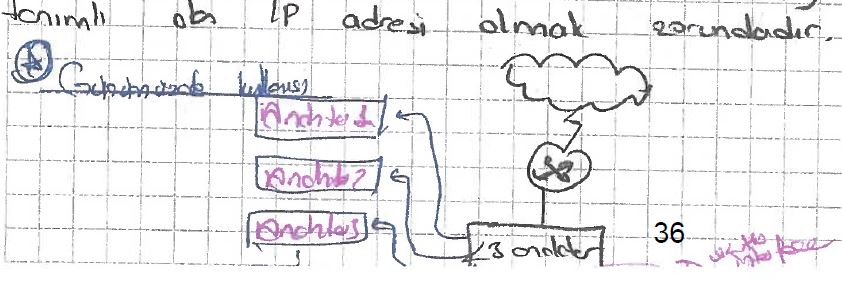
\includegraphics[width=10cm]{
images/sayfa36sonresim} \label{fig:Şirket örneği 2} \end{figure}

\underline{Soruya gelirsek : }

\begin{tabular}{|c|c|}
\hline
128 Teknik Birim 
&
\begin{tabular}{c|c}
\multicolumn{2}{c}{64 Pazarlama} \\
\hline
32 Muhasebe & 32 İdari birim \\

\end{tabular}\\
\hline
\end{tabular}

Ağ adresi : 192.168.0.0

Yayın adresi : 192.168.100.127

\begin{tabular}{|c|c|}
\hline
Teknik  
&
\begin{tabular}{l}
192.168.100.0(Ağ adresi) \\
192.168.100.127(Yayın adresi)
\end{tabular}\\
\hline
\end{tabular}

\begin{tabular}{|c|c|}
\hline
Pazarlama  
&
\begin{tabular}{l}
192.168.100.128 \\
192.168.100.191 \\
\end{tabular}\\
\hline
\end{tabular}

\begin{tabular}{|c|c|}
\hline
Muhasebe  
&
\begin{tabular}{l}
192.168.100.192 \\
192.168.100.223 \\
\end{tabular}\\
\hline
\end{tabular}

\begin{tabular}{|c|c|}
\hline
İdari birim
&
\begin{tabular}{l}
192.168.100.224 \\
192.168.100.255\\
\end{tabular}\\
\hline
\end{tabular}

Alt ağ maskesi ise teknik:255.255.255.0,

 pazarlama:255.255.255.192,
 
  muhasebe:255.255.255.224,
  
   idari:255.255.255.255 ??? şeklindedir. 
   
\textbf{ÖRNEK : } 10.50.100.200/25 şeklinde IP adresi tahsis edilmiş bir bilgisayarın ağ adresi ve yayın adresi nedir? 

32-25=7 olduğundan  $2^7 =128$ tane IP var. 

\begin{tabular}{lll}
 & 10.50.100.200 &\\
x&255.255.255.128& \\
\hline
 & 10.50.100.128 & ağ adresi \\
 & 10.50.100.255 & yayın adresi 
\end{tabular}    

\textbf{ÖRNEK : } Aşağıdaki bilgisayarlardan hangileri ağ geçidine ihtiyaç duymadan haberleşirler. 

\begin{center}
\begin{tabular}{rlrl}
   &               &\underline{Ağ adresi} & \\
a) & 10.0.0.120/25 & 10.0.0.0 & -128 \\
b) & 10.0.0.121/24 & 10.0.0.0 & -256 \\
c) & 10.0.0.254/24 & 10.0.0.0 & -256 \\
d) & 10.0.0.1/24 & 10.0.0.0 & -256 \\
e) & 10.0.0.253/25 & 10.0.0.0 & -128 \\

\end{tabular}

\end{center}

\textbf{NOT : } X'in Y ile aynı ağda olup olmadığını anlamak için X bilgisayarı Y nin IP adresiyle kendi ağ maskesini çarpar. Kendi ağ adresiyle karşılaştırır. 

A'nın B ile haberleşmesi : 

\begin{tabular}{lllll}
B'nin IP adresi & &10.0.0.121 &\\
A'nın ağ maskesi &x&10.0.0.128& \\
\hline 
 & & 10.0.0.0 & \\
\end{tabular} 

Çıkan sonuç A'nın ağ adresiyle aynı olduğundan haberleşirler. 

A'nın C ile haberleşmesi : 

\begin{tabular}{lllll}
C'nin IP adresi & &10.0.0.254 &\\
A'nın ağ maskesi &x&10.0.0.128& \\
\hline 
 & & 10.0.0.128 & \\
\end{tabular} 

Çıkan sonuç A'nın ağ adresiyle aynı olmadığından haberleşemezler.